\chapter{Lögmál Faradays og spanstraumur}

\section{Lögmál Faradays}

\begin{tcolorbox}
\begin{theorem}
\textbf{(Lögmál Faradays)} Breyting á segulflæði, $\frac{d\Phi_B}{dt}$, spanar spanspennu, $\mathcal{E}(t)$, og spanstraum $J(t)$, samkvæmt:
\begin{align*}
    R J(t) = \mathcal{E}(t) = \oint \Vec{E} \cdot d\vec{\ell} = -\frac{d\Phi_B}{dt}.
\end{align*}
Þar sem að $R$ er viðnámið í rásinni þar sem að spanstraumurinn spanast.
\end{theorem}
\end{tcolorbox}


Þar sem að segulflæðið er gefið með $\Phi_B = \vec{B} \cdot \vec{A} = BA\cos\gamma$ þar sem að $\gamma$ er hornið á milli vigranna. Ef $\gamma = \ang{0}$ þá eru aðallega tvær leiðir fyrir okkur til þess að breyta seglflæðinu. Við höfum nefnilega samkvæmt diffrun margfeldis að:
\begin{align*}
    \frac{d\Phi_B}{dt} = \frac{d}{dt}\left( BA \right) = \frac{dB}{dt} A + B \frac{dA}{dt}
\end{align*}
Í flestum dæmum sem að við munum skoða þá er annaðhvort $\frac{dA}{dt} = 0$ eða $\frac{dB}{dt} = 0$ svo að við höfum annað hvort að:
\begin{align*}
    \frac{d\Phi_B}{dt} = A \frac{dB}{dt}, \hspace{1cm} \text{eða} \hspace{1cm} \frac{d\Phi_B}{dt} = B \frac{dA}{dt}.
\end{align*}
Með öðrum orðum þá er það annaðhvort segulsviðið sem að breytist með tíma eða flatarmálið sem að breytist með tíma. Reyndar ættum við að nefna að stundum er það hornið $\gamma$ á milli vigranna sem er breytt (með því að snúa gjörð með fast flatarmál $A$ í föstu segulsviði $B$) þá fæst:
\begin{align*}
    \frac{d\Phi_B}{dt} = \frac{d}{dt}\left( BA \cos\gamma \right) = -BA\sin\gamma \frac{d\gamma}{dt} = -\omega BA \sin\gamma(t)
\end{align*}
Þar sem að $\omega = \frac{d\gamma}{dt}$ er hornhraðinn sem að gjörðinni er snúið með.

\newpage

\section{Sýnidæmi}

Skoðum til dæmis uppstillinguna á myndinni hér fyrir neðan:

\begin{figure}[H]
    \centering
    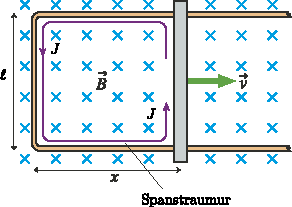
\includegraphics{figures/rk3026.pdf}
\end{figure}

Búið er að koma fyrir rennivír ofan á $U$-laga vír. Það er einsleitt segulsvið, $\vec{B}$, inn í töfluna. Rennivírinn lokar rásinni þannig að flatarmál rásarinnar þar sem að straumurinn getur hlaupið er $A = \ell x$ þar sem að $x$ er fjarlægðin sem að rennivírinn hefur verið dreginn. Vírarnir hafa eðlisviðnám $\rho$ og rennivírinn hefur viðnám $R_r$. Nú byrjum við að draga rennivírinn til hægri með hraða $v$. Þá breytist flatarmál gjarðarinnar (en segulsviðið er óbreytt svo $\frac{dB}{dt} = 0$) og flatarmálið er þá gefið með:
\begin{align*}
    A(t) = \ell (x_0 + vt) = \ell x_0 + \ell vt
\end{align*}
þar sem $x_0$ er fjarlægð rennivírsins frá vinstri endanum í byrjun. En þá fáum við að:
\begin{align*}
    \frac{d \Phi_B}{dt} = \frac{d}{dt}\left( BA \right) = B \frac{dA}{dt} = B\ell v
\end{align*}
En samkvæmt lögmáli Faradays er þá spanspennan sem að spanast gefin með:
\begin{align*}
    \mathcal{E}(t) = - \frac{d\Phi_B}{dt} = - B\ell v
\end{align*}
Við getum hunsað mínusmerkið því það er einungis notað til þess að segja okkur í hvaða stefnu straumurinn spanast. Núna er segulflæðið að aukast inn í blaðið (því $\vec{B}$ er inn í blaðið og $A$ er að aukast) svo að við ályktum að straumurinn spanast rangsælis (miðað við klukkuganginn) í rásinni. Straumurinn í rásinni verður þá gefinn með:
\begin{align*}
    \left(R_r + \rho \cdot \frac{\ell + 2x(t)}{A}\right)J(t) = Blv \implies J(t) = \frac{Blv}{R_r + \rho \frac{\ell + 2x_0}{A} + \rho \frac{2vt}{A}}
\end{align*}
Þar sem að $A$ er þverskurðarflatarmál $U$-laga vírsins. Sér í lagi sjáum við að $J(t) \xrightarrow[t \to +\infty] \ 0$. \\

Annað sem maður gæti spurt að er hversu mikil orka tapast þá út um $R_r$ viðnámið. Við athugum þá að:
\begin{align*}
    P = I \Delta V_{R_r} = I^2 R_r \implies P(t) = J^2(t) R_r.
\end{align*}
Heildaraflið sem tapast í rásinni er hinsvegar:
\begin{align*}
    P = J(t)\mathcal{E}(t).
\end{align*}

\newpage

\section{Sjálfspan í spólu}

\begin{tcolorbox}
\begin{theorem}
\textbf{(Spanstuðull)} Við skilgreinum spanstuðul spólu þannig að spennufallið yfir spóluna, $\Delta V_L$, er gefið með:
\begin{align*}
    \Delta V_L = - L \frac{dI}{dt}.
\end{align*}
\end{theorem}
\end{tcolorbox}

\begin{tcolorbox}
\begin{theorem}
\textbf{(Sjálfspan spólu)} Lítum á spólu með geisla $R$ af lengd $\ell$ og með vafningafjölda $N$. Þá er spanstuðull spólunnar gefinn með:
\begin{align*}
    L_{\text{langspóla}} = \frac{\mu_0 A N^2}{\ell},
\end{align*}
þar sem $A = \pi R^2$.
\end{theorem}
\end{tcolorbox}

\textbf{Útleiðsla:} Við höfum að segulflæðið í einni lykkju breytist samkvæmt:
\begin{align*}
    \frac{d\Phi_B}{dt} = \frac{d}{dt}\left( BA \right) = A \frac{d}{dt}(B) = A \frac{d}{dt}\left( \frac{\mu_0 I N}{\ell} \right) = \frac{\mu_0 A N}{\ell} \frac{dI}{dt}.
\end{align*}
En það eru alls $N$ lykkjur og hver þeirra veitir sama framlag til spanspennunar svo að við jöfum að spennufallið er:
\begin{align*}
    \Delta V_L = \mathcal{E}(t) = -N \cdot \frac{d \Phi_B}{dt} = - \frac{\mu_0 A N^2}{\ell} \frac{dI}{dt} = -L \frac{dI}{dt} \implies L_{\text{langspóla}} = \frac{\mu_0 A N^2}{\ell}.
\end{align*}
Þar sem að $A = \pi R^2$ er þverskurðarflatarmál spólunnar. \qed




\begin{tcolorbox}
\begin{theorem}
\textbf{(Orkuþéttleiki segulsviðsins)} Orkuþéttleiki (orka á rúmmálseiningu) segulsviðs er gefið með:
\begin{align*}
    u_B = \frac{1}{2\mu_0}B^2.
\end{align*}
\end{theorem}
\end{tcolorbox}

Til samanburðar var orkuþéttleiki rafsviðsins:
\begin{align*}
    u_E = \frac{1}{2}\varepsilon_0 E^2.
\end{align*}



\begin{tcolorbox}
\begin{theorem}
\textbf{(Orkan í spólu)} Orkan sem að spóla með spanstuðul $L$ geymir þegar að straumur $I$ fer í gegnum hana er gefin með:
\begin{align*}
    U_L = \frac{1}{2}LI^2.
\end{align*}
\end{theorem}
\end{tcolorbox}

\textbf{Útleiðsla:} Orkuþéttleiki segulsviðsins er:
\begin{align*}
    u_B = \frac{1}{2\mu_0}B^2
\end{align*}
En þar með höfum við að orkan sem að spólan geymir er:
\begin{align*}
   U_L =  u_B \cdot A \ell = \frac{1}{2\mu_0} \left( \frac{\mu_0 I N}{\ell} \right)^2 A \ell = \frac{1}{2} \cdot \frac{\mu_0 A N^2}{\ell} \cdot I^2 = \frac{1}{2}L I^2. \qed
\end{align*}

\section{Hvers vegna er riðstraumur málið?}

Skoðum eftirfarandi uppstillingu:

\begin{figure}[H]
    \centering
    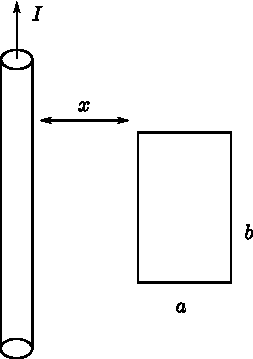
\includegraphics{figures/straumur-vir.pdf}
\end{figure}

Vír ber straum $I$ upp og rétthyrningslaga gjörð með hliðarlengdir $a$ og $b$ er stödd í fjarlægð $x$ frá vírnum. Til að byrja með ætlum við að skoða hvað gerist þegar að straumurinn er fastur (þ.e.a.s. frá jafnspennugjafa). Athugum að vírinn býr til segulsvið í kringum sig og að segulsviðið er því missterkt eftir því hvar við erum í gjörðinni. Við höfum þá að heildarsegulflæðið út um gjörðina er:
\begin{align*}
    B(r) = \frac{\mu_0 I}{2\pi r}, \hspace{0.5cm} \text{þannig að:} \hspace{0.5cm}
    \Phi_B = \int_{x}^{x+a} \frac{\mu_0 I}{2\pi r} b dr = \left[ \frac{\mu_0 I}{2\pi} \ln(r) \right]_{x}^{x+a} = \frac{\mu_0 I}{2\pi} \ln(\frac{x+a}{x}) = \frac{\mu_0 I}{2\pi} \ln(1 + \frac{a}{x})
\end{align*}
Þetta er óháð því hvort að straumurinn er tímaháður eða ekki. Ef $I$ er fast þá fæst einfaldlega að:
\begin{align*}
    \frac{d\Phi_B}{dt} = 0.
\end{align*}
En þar með spanast enginn straumur í rásinni ef að við erum með jafnan straum. Hinsvegar ef að við erum með riðstraum, $I(t) = I_0 \sin(\omega t)$ þá höfum við að:
\begin{align*}
    \frac{d \Phi_B}{dt} = \frac{d}{dt}\left( \frac{\mu_0 I(t)}{2\pi} \ln(1 + \frac{a}{x}) \right) = -\frac{\mu_0 I_0 \omega}{2 \pi} \ln(1 + \frac{a}{x}) \cos(\omega t)
\end{align*}
Ef að heildarviðnám gjarðarinnar er $R$ þá fáum við að spanstraumurinn sem að spanst í rásinni er gefinn með:
\begin{align*}
    R J(t) = \mathcal{E}(t) = -\frac{d\Phi_B}{dt} = \frac{\mu_0 I_0 \omega}{2 \pi} \ln(1 + \frac{a}{x}) \cos(\omega t) \implies J(t) = \frac{\mu_0 I_0 \omega}{2 \pi R} \ln(1 + \frac{a}{x}) \cos(\omega t)
\end{align*}


\newpage

\section{Dæmi}

\subsection*{Dæmatími 24: Lögmál Faradays og lögmál Lenz}

\begin{tcolorbox}
Lögmál Faradays segir að spanspennan sem að myndast við það að segulflæði breytist er gefið með:
\begin{align*}
     \mathcal{E}(t) = \int \vec{E} \cdot d\vec{\ell} = -\frac{d \Phi_B}{dt}
\end{align*}
 En spanspennan getur myndað spanstraum, $J(t)$ í rás sem hefur viðnám $R$ samkvæmt:
\begin{align*}
     \mathcal{E}(t) = J(t) R.
\end{align*}
Mínusmerkið í lögmáli Faradays hefur fengið sérstakt nafn og kallast lögmál Lenz. Það segir að spanstraumurinn sem að myndast í rásinni er í öfuga átt miðað við breytinguna á segulflæðinu.
\end{tcolorbox}

\begin{enumerate}[label = \textbf{(\alph*)}]

\item[\textbf{(30.11)}] Helmingurinn af einshliða þríhyrning með $\SI{20}{cm}$ hliðarlengdir er staddur inni í segulsviði sem að hefur styrk \SI{0.10}{T}. \begin{enumerate*}[label = \textbf{(\alph*)}]
    \item Hvert er segulflæðið út um þríhyrninginn?
    \item Þríhyrningurinn er búinn til úr koparvír sem hefur geisla $\SI{1.5}{mm}$. Hvert er viðnám þríhyrningsins? Eðlisviðnám kopars er $\SI{1.7e-8}{\ohm.m}$.
    \item Segulsviðið byrjar skyndilega að minnka um \SI{0.01}{T/s}. Hver er stærð og stefna spanstraumsins sem að spanast í rásinni?
\end{enumerate*}

\item[\textbf{(30.13)}] Rétthyrningslaga gjörð er ýtt inn í einsleitt \SI{0.20}{T} segulsvið með hraðanum \SI{50}{m/s}. Viðnám gjarðarinnar er \SI{0.10}{\ohm}. Hver er stærð og stefna spanstraumsins sem að spanast í rásinni?

\item[\textbf{(30.15)}] Ferningslaga gjörð með hliðarlengdir \SI{8.0}{cm} hefur viðnám \SI{0.20}{\ohm}. Á myndinni sést að spanstraumurinn í rásinni er \SI{150}{mA}. Er styrkur segulsviðsins að aukast eða að minnka (inn í blaðið)? Með hvaða hraða (\si{T/s}) er styrkur segulsviðsins að breytast?

\item[\textbf{(30.14)}] Allar gjarðirnar í liðum \textbf{(a)}, \textbf{(b)} og \textbf{(c)} hafa \SI{10}{cm} þvermál og eru staddar í þremur mismunandi segulsviðum. Viðnám gjarðanna er \SI{0.20}{\ohm}. Hver er stærð og stefna spanstraumsins sem að spanast í gjörðunum þremur?


\end{enumerate}

\begin{figure}[H]
    \centering
    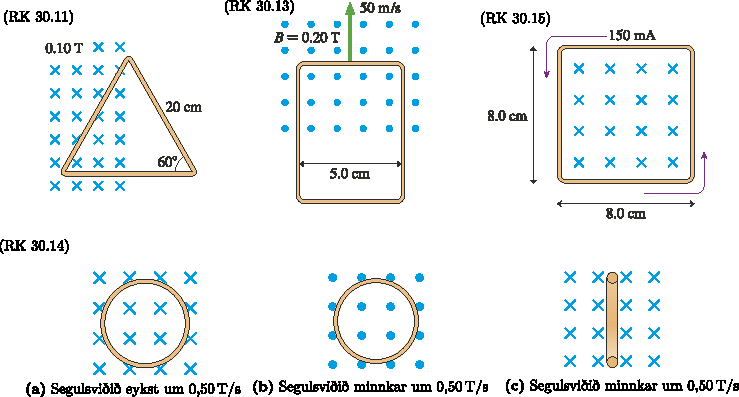
\includegraphics[scale = 1.15]{figures/rk3011.pdf}
\end{figure}

\begin{tcolorbox}
\begin{enumerate*}[label = ]
  \item \textbf{(30.11)} $J = \SI{1.2}{mA}$.
  \item \textbf{(30.13)} $J = \SI{5.0}{A}$.
  \item \textbf{(30.15)} $\frac{dB}{dt} = \SI{4.7}{\frac{T}{s}}$.
  \item \textbf{(30.14)} $J_a = J_b = \SI{20}{mA}$.
\end{enumerate*}
\end{tcolorbox}


\newpage

\subsection*{Dæmatími 25: Spanstraumur}

\begin{enumerate}[label = \textbf{(\alph*)}]

\begin{minipage}{\linewidth}
\begin{wrapfigure}{r}{1.5in}
\vspace{-0.75cm}
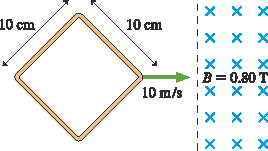
\includegraphics[width = 2in]{figures/rk3053b.pdf}
\end{wrapfigure}

\item[\textbf{(30.53)}] Ferningslaga gjörð hefur hliðarlengdir $ \SI{10}{cm}$ og ferðast inn í einsleitt \SI{0.80}{T} segulsvið með hraða \SI{10}{m/s}. Viðnám gjarðarinnar er \SI{0.10}{\ohm}. \begin{enumerate*}[label = \textbf{(\alph*)}]
    \item Teiknið graf sem sýnir spanstrauminn í rásinni, $J(t)$, sem fall af tíma, $t$ frá $t = \SI{0.000}{s}$ til $t = \SI{0.020}{s}$.
    \item Hver verður mesti straumurinn í rásinni? Hvar er gjörðin stödd þegar að straumurinn er mestur?
\end{enumerate*}

\end{minipage}

\vspace{0.3cm}

\begin{minipage}{\linewidth}
\begin{wrapfigure}{r}{1.5in}
\vspace{-0.25cm}
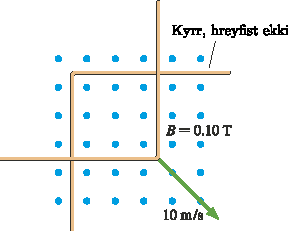
\includegraphics[width = 2in]{figures/rk3054.pdf}
\end{wrapfigure}

\item[\textbf{(30.54)}] Tveir L-laga vírar sjást á myndinni hér til hægri. Þeir eru staddir í einsleitu \SI{0.10}{T} segulsviði. Við tímann $t = \SI{0}{s}$ þá eru hornpunktar þeirra staddir í sama punkti (flatarmálið sem að vírarnir umlykja er þá núll í byrjun). Þá byrjum við að draga annan L-laga vírinn með hraða \SI{10}{m/s} undir \ang{45} horni miðað við lárétt á meðan að við höldum hinum vírnum kyrrum. Vírarnir, sem eru úr gulli, hafa eðlisviðnám $\rho_{\text{gull}} = \SI{2.4e-8}{\ohm.m}$ og þvermál $\SI{1.75}{mm}$. \begin{enumerate*}[label = \textbf{(\alph*)}]
    \item Hver er stefna spanstraumsins í rásinni?
    \item Ákvarðið spanspennuna, $\mathcal{E}(t)$ og spanstrauminn, $J(t)$, sem fall af tíma, $t$.
    \item Gefið töluleg gildi á spanspennunni og spanstraumnum við tímann $t = \SI{0.10}{s}$.
\end{enumerate*}

\end{minipage}

\vspace{0.3cm}


\begin{minipage}{\linewidth}
\begin{wrapfigure}{r}{1.5in}
\vspace{-0.25cm}
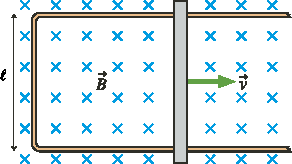
\includegraphics[width = 2in]{figures/rk3026b.pdf}
\end{wrapfigure}

\item[\textbf{(30.55)}]  Rennivír nokkur er $\SI{20}{cm}$ að lengd og hefur massa \SI{50}{mg} og viðnám \SI{1.0}{\ohm}. Rennivírinn er dreginn með föstum hraða \SI{10}{m/s} til hægri í einsleitu \SI{0.10}{T} segulsviði eins og sést á myndinni hér til hægri. Rennivírinn rennur meðfram núningslausum, ofurleiðandi teinum sem hafa ekkert viðnám (eina viðnámið í rásinni er þá vegna rennivírsins). \begin{enumerate*}[label = \textbf{(\alph*)}]
    \item Hver er spanstraumurinn sem að spanast í rásinni?
    \item Hversu mikinn kraft þarf til þess að draga vírinn?
    \item Þegar að vírinn er dreginn svona mun spanstraumurinn í rásinn valda því að varmaafl tapast í viðnámi rennivírsins og hann mun þar af leiðandi hitna. Eðlisvarmi vírsins er $c_{\!_\text{Kopar}} = \SI{710}{J/kg.K}$. Um hversu margar gráður hitnar rennivírinn við það að draga hann svona í \SI{10}{s}?
\end{enumerate*}

\end{minipage}

\vspace{0.3cm}

%\item[\textbf{(30.58)}]


\begin{minipage}{\linewidth}
\begin{wrapfigure}{r}{1in}
\vspace{-1.25cm}
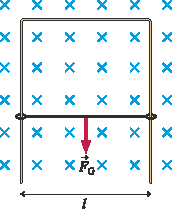
\includegraphics[width = 1.2in]{figures/rk3059.pdf}
\end{wrapfigure}

\item[\textbf{(30.59)}] Rennivír nokkur er \SI{20}{cm} að lengd og hefur massa \SI{10}{g} og viðnám \SI{0.10}{\ohm}. Rennivírinn getur runnið lóðrétt meðfram U-laga núningslausum, ofurleiðandi teinum eins og sést á myndinni hér til hægri. Styrkur segulsviðsins er \SI{0.50}{T}. Nú er kerfinu sleppt úr kyrrstöðu og þyngdarkrafturinn sem að verkar á rennivírinn togar hann þá niður. Eftir einhvern tíma mun rennivírinn vera í kraftjafnvægi og ferðast þá með föstum lokahraða niður, $v_{\text{lok}}$. Ákvarðið lokahraðann.

\end{minipage}

\end{enumerate}

\vspace{1cm}

\begin{tcolorbox}
\begin{enumerate*}[label = ]
  \item \textbf{(30.53)} $J_{\text{max}} = \SI{11.3}{A}$.
  \item \textbf{(30.54)} $\mathcal{E}(\SI{0.1}{s}) = \SI{1.0}{V}$, $J(\SI{0.1}{s}) = \SI{35.4}{A}$.
  \item \textbf{(30.55)} $J = \SI{0.20}{A}$, $F = \SI{4.0}{mN}$, $\Delta T = \SI{11.3}{\celsius}$
  \item \textbf{(30.59)} $v_{\text{lok}} = \SI{0.98}{m/s}$.
\end{enumerate*}
\end{tcolorbox}

\newpage


\subsection*{Dæmatími 26: Spanspólur og orkan í segulsviði}

\begin{tcolorbox}
Spanstuðull langspólu af lengd $\ell$ með vafningafjölda $N$ og þverskurðarflatarmál $A$ er gefinn með:
\begin{align*}
    L = \frac{\mu_0 N^2 A}{\ell}
\end{align*}
Spennufallið í gegnum spóluna er þá $\Delta V_L = - L \frac{dI}{dt}$. Orkan sem að spólan geymir er þá gefin með:
\begin{align*}
    U_L = \frac{1}{2}LI^2
\end{align*}
Orkuþéttleiki segulsviðsins er: $u_B = \frac{U_L}{A\ell} = \frac{1}{2\mu_0}B^2$.
\end{tcolorbox}


\begin{enumerate}[label = \textbf{(\alph*)}]

\item[\textbf{(30.12)}] Spansóla er búin til með því að vefja vír með þvermál \SI{0.30}{mm} þétt í kringum sívalning með geisla \SI{2.0}{mm}. \begin{enumerate*}[label = \textbf{(\alph*)}]
    \item Hversu löng þarf spólan að vera til þess að spanstuðull spólunnar sé \SI{10}{\mu H}?
    
    \item Nú hleypur fastur \SI{100}{mA} straumur í gegnum spóluna. Hversu mikla orku geymir spanspólan?
    
    \item Hver er orkuþéttleiki segulsviðsins inni í spólunni?
    
    \item Hver er styrkur segulsviðsins inni í spólunni?
    
    \item Skyndilega fellur straumurinn í spólunni niður í \SI{0}{A} á \SI{5.0}{\mu s}. Hvert var spennufallið yfir spóluna á meðan að straumurinn var að minnka?
\end{enumerate*}

\item[\textbf{(30.26)}] Spanspóla nokkur hefur spanstuðul \SI{100}{mH} og heildarviðnám vírsins sem að spólan er búin til úr er \SI{4.0}{\ohm}. Spólan er tengd við rafhlöðu sem hefur íspennu \SI{12}{V} og innra viðnám \SI{2.0}{\ohm}. Hversu mikla orku geymir spólan?

\item[\textbf{(30.27)}] Spóla nokkur er \SI{12}{cm} löng og hefur þvermál \SI{3.0}{cm} og vafningafjölda \SI{200}{}. Hversu mikla orku geymir spólan þegar að um hana streymir \SI{0.80}{A} rafstraumur?

\item[\textbf{(30.28)}] Segulómunartæki (MRI scanner) eru notuð í læknisfræðilegum tilgangi til þess að taka sneiðmyndir af líkamshlutum sjúklinga. Sá líkamshluti sem á að rannsaka er þá settur í miðju myndatökuklefans sem er í rauninni risastór spóla sem er \SI{40}{cm} í þvermál og \SI{1.0}{m} löng. Segulsviðið sem að myndast inni í myndatökuklefanum er \SI{5.0}{T} og er búið til með því að leiða \SI{100}{A} straum í gegnum spóluna. En eins og við höfum lært í verklegu þá getur stafað brunahætta af því að nota rafstraum sem er við meira en \SI{1.0}{A}. Af öryggisráðstöfun er því notast við ofurflæðandi helíum við lágt hitastig til þess að kæla vírana sem að spólan er búin til úr þannig að þeir vírar verða ofurleiðandi og hafa því svo gott sem ekkert innra viðnám.
\begin{enumerate*}[label = \textbf{(\alph*)}]
    \item Hver er vafningafjöldi spólunnar?
    \item Hversu mikla orku geymir spólan þegar hún er að myndgreina líkamshluta sjúklings?
    \item Hver er orkuþéttleiki segulsviðsins inni í myndatökuklefanum?
\end{enumerate*}


\end{enumerate}


\begin{tcolorbox}
\begin{enumerate*}[label = ]
  \item \textbf{(30.12)} $\ell = \SI{5.70}{cm}$, $U_L = \SI{5.0e-8}{J}$, $u_B = \SI{0.070}{J/m^3}$, $B = \SI{419}{\mu T}$, $\Delta V_L = \SI{0.20}{V}$.
  \item \textbf{(30.26)} $U_L = \SI{0.20}{J}$.
  \item \textbf{(30.27)} $L = \SI{296}{\mu H}$, $U_L = \SI{94.7}{\mu J}$.
  \item \textbf{(30.28)} $N = \SI{39800}{vafningar}$, $U_L = \SI{1.25}{MJ}$, $u_B = \SI{1.0e-7}{J/m^3}$.
\end{enumerate*}
\end{tcolorbox}

\newpage